%% Copyright 2018 H.\ Rabus
%
% This work may be distributed and/or modified under the
% conditions of the LaTeX Project Public License, either version 1.3
% of this license or (at your option) any later version.
% The latest version of this license is in
%   http://www.latex-project.org/lppl.txt
% and version 1.3 or later is part of all distributions of LaTeX
% version 2005/12/01 or later.
%
% This work has the LPPL maintenance status `author-maintained'.
%
% This work consists of the file texbsp.tex
%

\documentclass[smallheadings]{scrartcl}

%%% GENERAL PACKAGES %%%%%%%%%%%%%%%%%%%%%%%%%%%%%%%%%%%%%%%%%%%%%%%%%%%%%%%%%%
% inputenc allows the usage of non-ascii characters in the LaTeX source code
\usepackage[utf8]{inputenc}
\usepackage{graphicx} 
\usepackage{float}
%\graphicspath{ {/u/hnatiuka/Praktikum/PPI/} }



% title of the document
\title{Bericht zu Serie 2}
% optional subtitle
%\subtitle{Draft from~\today}
% information about the author
\author{%
  Arsen Hnatiuk,\\%
  Max Huneshagen 
}
\date{\today} 


%%% LANGUAGE %%%%%%%%%%%%%%%%%%%%%%%%%%%%%%%%%%%%%%%%%%%%%%%%%%%%%%%%%%%%%%%%%%
% babel provides hyphenation patterns and translations of keywords like 'table
% of contents'
\usepackage[ngerman]{babel}

%%% HYPERLINKS %%%%%%%%%%%%%%%%%%%%%%%%%%%%%%%%%%%%%%%%%%%%%%%%%%%%%%%%%%%%%%%%
% automatic generation of hyperlinks for references and URIs
\usepackage{hyperref}

%%% MATH %%%%%%%%%%%%%%%%%%%%%%%%%%%%%%%%%%%%%%%%%%%%%%%%%%%%%%%%%%%%%%%%%%%%%%
% amsmath provides commands for type-setting mathematical formulas
\usepackage{amsmath}
% amssymb provides additional symbols
\usepackage{amssymb}
% HINT
% Use http://detexify.kirelabs.org/classify.html to find unknown symbols!

%%% COLORS %%%%%%%%%%%%%%%%%%%%%%%%%%%%%%%%%%%%%%%%%%%%%%%%%%%%%%%%%%%%%%%%%%%%
% define own colors and use colored text
\usepackage[pdftex,svgnames,hyperref]{xcolor}

%%% Code Listings %%%%%%%%%%%%%%%%
% provides commands for including code (python, latex, ...)
\usepackage{listings}
\definecolor{keywords}{RGB}{255,0,90}
\definecolor{comments}{RGB}{0,0,113}
\definecolor{red}{RGB}{160,0,0}
\definecolor{green}{RGB}{0,150,0}
\lstset{language=Python, 
        basicstyle=\ttfamily\small, 
        keywordstyle=\color{keywords},
        commentstyle=\color{comments},
        stringstyle=\color{red},
        showstringspaces=false,
        identifierstyle=\color{green},
        }


\usepackage{paralist}
\usepackage{nicefrac}
% setting the font style for input und returns in description items
\newcommand{\initem}[2]{\item[\hspace{0.5em} {\normalfont\ttfamily{#1}} {\normalfont\itshape{(#2)}}]}
\newcommand{\outitem}[1]{\item[\hspace{0.5em} \normalfont\itshape{(#1)}]}
\newcommand{\bfpara}[1]{
	
	\noindent \textbf{#1:}\,}


\begin{document}

% generating the title page
\maketitle
% generating the table of contents (requires to run pdflatex twice!)
\tableofcontents
\bigskip

\hrule
\hrule

%%% BEGIN OF CONTENT %%%%%%%%%%%%%%%%%%%%%%%%%%%%%%%%%%%%%%%%%%%%%%%%%%%%%%%%%%

\section{Einleitung}

Das analytische Lösen von partiellen Differentialgleichungen kann manchmal schwierig, und oft unmöglich sein.

\section{Theorie}

\subsection{Speicherplatzbedarf}
\label{sec:bedarf}
Der wesentliche Unterschied zwischen vollbesetzten und \textit{sparse}-Matrizen  liegt in dem Speicherbedarf. Während eine vollbesetzte Matrix alle Einträge wie in einem Array speichert, werden nur die nicht-Null Einträge in einer \textit{sparse}-Matrix gespeichert. Also braucht eine $n \times n$ \textit{numpy.matrix} $n^2$ \textit{float}-Speicherplätze, jeweils \textit{64-bit}. Ein \textit{scipy.sparse.dok\_matrix}-Objekt  ist ein Wörterbuch-Objekt, dessen Schlüssel die \textit{(Zeile, Spalte)}-Koordinaten, und dessen Werte die Matrixeinträge sind. Also brauchen $n$ nicht-Null Einträge $2n$ \textit{int}Speicherplätze (für die zwei Schüssel-\textit{arrays}), jeweils \textit{24-bit}, und $n$ \textit{float}-Speicherplätze für den Matrixeintrag. Dagegen sind Keine Null Einträge gespeichert, also enthält das Wörterbuch die Schlüssel mit den Koordinaten der Null Einträge. Ein solches Objekt benutzt auch einen konstanten (also vernachlässigbaren) Speicherplatz für die Dimensionen der Matrix. Wir wenden nun die Speicherbedarfsanalyse auf eine Matrix wie in der Aufgabestellung mit Feinheit der Diskretisierung $n$ an. Wir approximieren dabei der Übersicht halber $2 \cdot 24 \approx 64$, um einen Wörterbuch-Eintrag als zwei \textit{float}-Einträge zu betrachten, damit nut \textit{float}-Speicherplätze in Frage kommen.

\paragraph{d = 1}
In der ersten Dimension hat die vollbesetzte Matrix $n^2$ Einträge, also einen Speicherbedarf der Ordnung $\mathcal{O}(n^2)$.

Die nicht-Null Einträge dieser Matrix stehen auf der drei zentralen Diagonalen. Also benötigt das \textit{scipy.sparse.dok\_matrix}-Objekt $2(n+2(n-1)) = \mathcal{O}(6n)$ Speicherplätze.

\paragraph{d = 2}
Die $d=2$-Matrix besteht aus $n^2$ Matrizen, die die gleiche Größe wie eine $d=1$-Matrix haben. Also ist der Speicherbedarf der \textit{numpy}-Matrix der Ordnung $\mathcal{O}(n^4)$.

 Diese Matrix hat $n$ viele $d=1$-Matrizen auf der Hauptdiagonale  und $2(n-1)$ Einheitsmatrizen auf den zwei Nebendiagonalen, mit jeweils $n$ nicht-Null Einträge. Insgesamt macht das $2(n(\mathcal{O}(6n))+2n(n-1))=\mathcal{O}(16n^2)$ Speicherplätze.
 
 \paragraph{d = 3}
 Die $d=3$-Matrix besteht aus $n^2$ Matrizen, die die gleiche Größe wie eine $d=2$-Matrix haben. Also ist der Speicherbedarf der \textit{numpy}-Matrix der Ordnung $\mathcal{O}(n^6)$.
 
 Die untersuchte Matrix hat $n$ viele $d=2$-Matrizen auf der Hauptdiagonale  und $2(n-1)$ Einheitsmatrizen auf den zwei Nebendiagonalen, mit jeweils $n^2$ nicht-Null Einträge. Insgesamt macht das $2(n(\mathcal{O}(16n^2))+2n^2(n-1))=\mathcal{O}(36n^3)$ Speicherplätze.

\section{Experiment}

In \textit{experimente.py} wird die relative Anzahl der Nicht-Null-Einträge der Matrix $A^{(d)}$ für $d=1,2,3$ numerisch untersucht und anschließend graphisch dargestellt. Darüber hinaus wird die Gesamtanzahl der Einträge einer vollbesetzen Matrix der gleichen Größe wie $A^{(d)}$ in Abhängigkeit von $n$ geplottet. Diese ergibt sich zu $(n-1)^{2d}$, da $A^{(d)}\in\mathbb{R}^{(n-1)^d\times(n-1)^d}$ Das Ergebnis des Experiments ist in Abb.~\ref{im:nn_eintr} doppeltlogarithmisch dargestellt.

\begin{figure}[H]
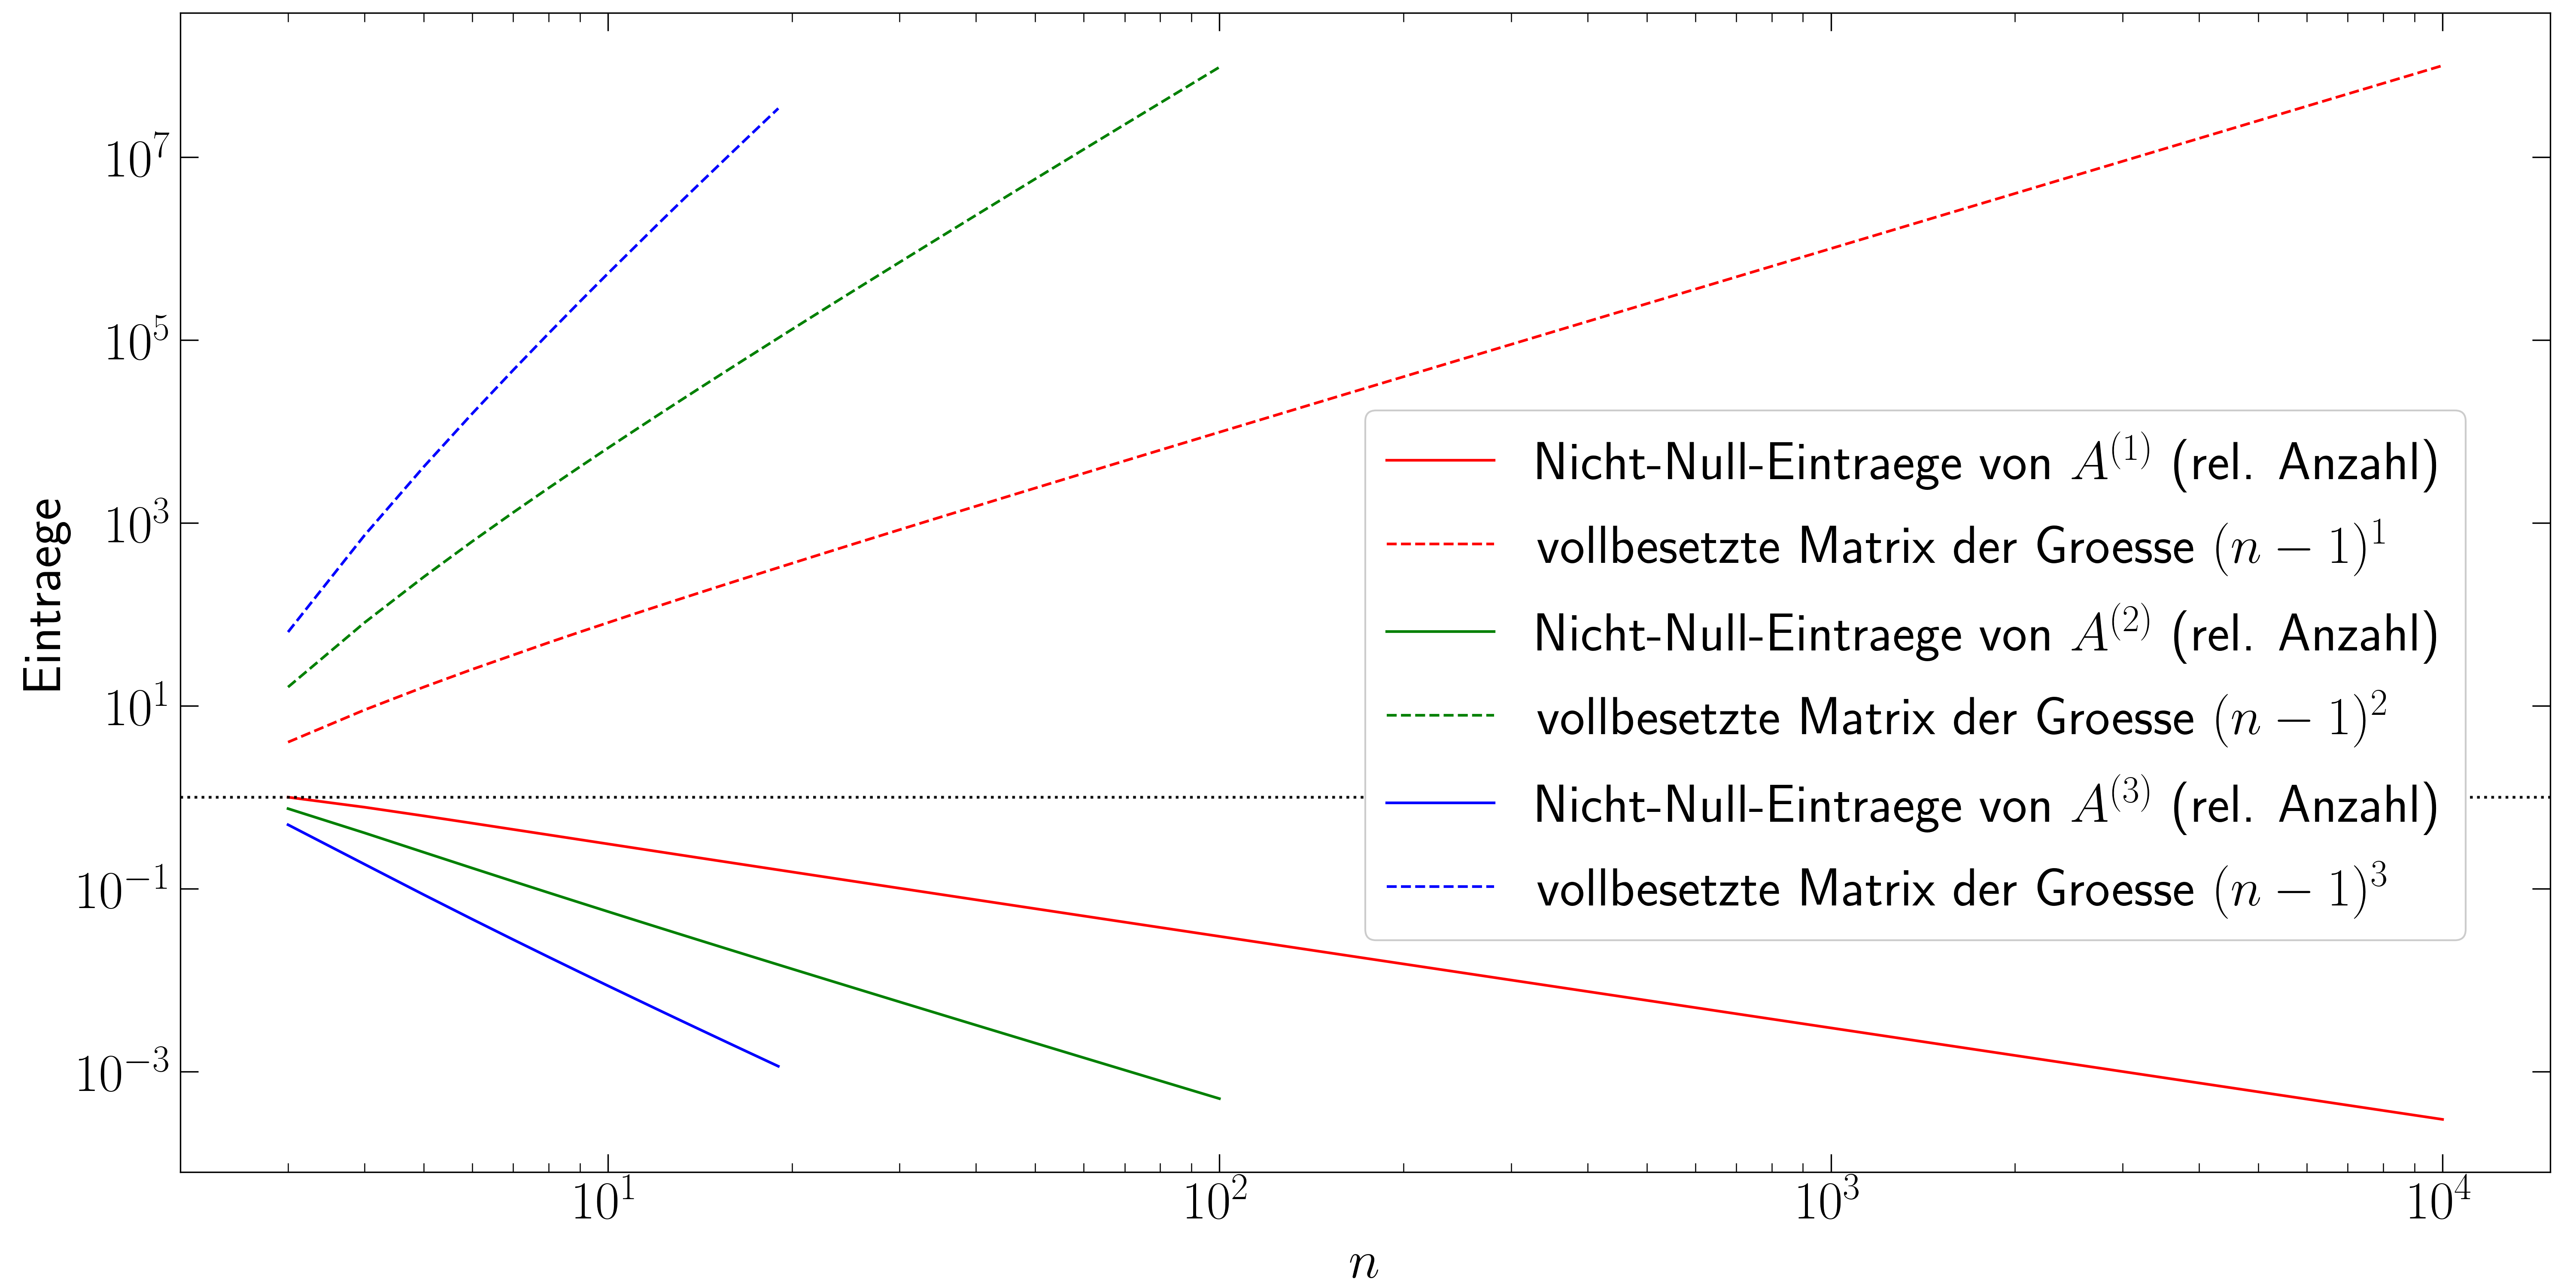
\includegraphics[width=\textwidth]{Bilder/nn_eintraege}

\caption{Durchgezogen: Nicht-Null-Einträge von $A^{(d)}$ für $d=1,2,3$ (relative Anzahl). Gestrichelt: Einträge einer vollbesetzten Matrix der gleichen Größe wie $A^{(d)}$.}
\label{im:nn_eintr}
\end{figure}



Man erkennt, dass die relative Anzahl der Nicht-Null-Einträge (und damit der Speicheraufwand des \textit{scipy.dok\_matrix}-Objektes für jedes untersuchte $d$ verschieden stark abfällt. Bezeichnet $a_{\text{nn},d}(n)$ die Anzahl der 
Nicht-Null-Einträge von $A^{(d)}$, so ergibt sich durch eine graphische Analyse, dass $a_{\text{nn},d}\sim n^{-d}$ wie in Abschnitt \ref{sec:bedarf} vorhergesagt. Mit zunehmender Feinheit der Diskretisierung wird die Matrix deutlich dünner besetzt und die Speicherung als Sparse-Matrix immer sinnvoller. Man beachte dazu insbesondere die zunehmende Differenz zum Wert 1, der in Abb.~\ref{im:nn_eintr} durch eine gepunktete Linie eingetragen wurde. 


\section{Zusammenfassung}


\begin{thebibliography}{9}
\bibitem{wiki} Kein Autor, Aufgerufen am 22.11.2018, \textit{Sparse Matrix}. 
\url{https://en.wikipedia.org/wiki/Sparse_matrix}
\end{thebibliography}


%%% END OF DOCUMENT %%%%%%%%%%%%%%%%%%%%%%%%%%%%%%%%%%%%%%%%%%%%%%%%%%%%%%%%%%%
\end{document}
